\subsection{Regular subclasses}
\label{subsec:library_of_transformations:type_level_transformations:regular_subclasses}

\begin{figure}[H]
    \centering
    \begin{subfigure}{0.4\textwidth}
        \centering
        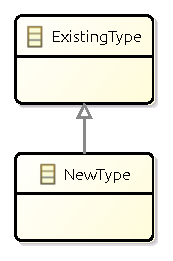
\includegraphics{images/05_library_of_transformations/02_type_level_transformations/03_regular_subclasses/class_subtype.pdf}
        \caption{$Tm_{Subclass}$ with $name = .\type{NewType}$ and $supertype = .\type{ExistingType}$}
        \label{fig:library_of_transformations:type_level_transformations:regular_subclasses:visualisation:ecore}
    \end{subfigure}
    \begin{subfigure}{0.4\textwidth}
        \centering
        % To use this figure in your LaTeX document
% import the package groove/resources/groove2tikz.sty
%
\begin{tikzpicture}[scale=\tikzscale,name prefix=test-]
\node[type_node] (n0) at (1.375, -1.525) {\ml{\textbf{NewType}}};
\node[type_node] (n1) at (1.365, -0.595) {\ml{\textbf{ExistingType}}};

\path[subtype_edge](n0.north -| 1.365, -0.595) --  (n1) ;
\end{tikzpicture}

        \caption{$TG_{Subclass}$ with $name = .\type{NewType}$ and $supertype = .\type{ExistingType}$}
        \label{fig:library_of_transformations:type_level_transformations:regular_subclasses:visualisation:groove}
    \end{subfigure}
    \caption{Visualisation of the transformation of regular subclasses}
    \label{fig:library_of_transformations:type_level_transformations:regular_subclasses:visualisation}
\end{figure}

This section will define the transformation of a regular subclass. Within this transformation, a newly introduced subclass is transformed, which extends an existing supertype. The Ecore type model that introduces such a subclass is defined as follows:

\begin{defin}[Type model $Tm_{Subclass}$]
\label{defin:library_of_transformations:type_level_transformations:regular_subclasses:tmod_subclass}
Let $Tm_{Subclass}$ be the type model containing a regular class with identifier $name$. The regular class $name$ extends another regular class with identifier $supertype$. Furthermore, $name \neq supertype$. $Tm_{Subclass}$ is defined as:
\begin{align*}
Class =\ &\{name, supertype\} \\
Enum =\ &\{\} \\
UserDataType =\ &\{\} \\
Field =\ &\{\} \\
\mathrm{FieldSig} =\ &\{\} \\
EnumValue =\ &\{\} \\
Inh =\ &\{(name, supertype)\} \\
Prop =\ &\{\} \\
Constant =\ &\{\} \\
\mathrm{ConstType} =\ &\{\}
\end{align*}
\isabellelref{tmod_subclass}{Ecore-GROOVE-Mapping-Library.SubclassType}
\end{defin}

\begin{thm}[Correctness of $Tm_{Subclass}$]
\label{defin:library_of_transformations:type_level_transformations:regular_subclasses:tmod_subclass_correct}
$Tm_{Subclass}$ (\cref{defin:library_of_transformations:type_level_transformations:regular_subclasses:tmod_subclass}) is a consistent type model in the sense of \cref{defin:formalisations:ecore_formalisation:type_models:type_model_consistency}.
\isabellelref{tmod_subclass_correct}{Ecore-GROOVE-Mapping-Library.SubclassType}
\end{thm}

A visual representation of $Tm_{Subclass}$ with the new subclass identified as $.\type{NewType}$ and the existing supertype identified as $.\type{ExistingType}$ can be seen in \cref{fig:library_of_transformations:type_level_transformations:regular_subclasses:visualisation:ecore}. The correctness proof of $Tm_{Subclass}$ is trivial, and therefore not included here. The proof can be found as part of the Isabelle validated proofs.

In order to make composing transformation functions possible, $Tm_{Subclass}$ should be compatible with the type model it is combined with.

\begin{thm}[Correctness of $\mathrm{combine}(Tm, Tm_{Subclass})$]
\label{defin:library_of_transformations:type_level_transformations:regular_subclasses:tmod_subclass_combine_correct}
Assume a type model $Tm$ that is consistent in the sense of \cref{defin:formalisations:ecore_formalisation:type_models:type_model_consistency}. Then $Tm$ is compatible with $Tm_{Subclass}$ (in the sense of \cref{defin:transformation_framework:type_models_and_type_graphs:combining_type_models:compatibility}) if:
\begin{itemize}
    \item The only shared type is the supertype, so $Class_{Tm} \cap Class_{Tm_{Subclass}} = \{ supertype \}$;
    \item The class $name$ is not in the namespace of class $supertype$, and vice versa;
    \item $name$ is not used as an identifier for an enumeration type or user-defined data type in $Tm$;
    \item The identifier of the class $name$ in $Tm_{Class}$ is not in the namespace of any class, enumeration type or user-defined data type in $Tm$;
    \item None of the identifiers in any class, enumeration type or user-defined data type in $Tm$ is in the namespace of the class $name$ in $Tm_{Class}$.
\end{itemize}
\isabellelref{tmod_subclass_combine_correct}{Ecore-GROOVE-Mapping-Library.SubclassType}
\end{thm}

\begin{proof}
Use \cref{defin:transformation_framework:type_models_and_type_graphs:combining_type_models:tmod_combine_merge_correct}. It is possible to show that all assumptions hold. For proving that the transitive closure of the inheritance relation is irreflexive, use the fact that $name$ only appears in the domain of the relation. Now we have shown that $\mathrm{combine}(Tm, Tm_{Class})$ is consistent in the sense of \cref{defin:formalisations:ecore_formalisation:type_models:type_model_consistency}.
\end{proof}

The definitions and theorems for a regular subclass within Ecore are now complete. 

\subsubsection{Encoding as node type}

A possible encoding for regular subclasses in Ecore is using node types in GROOVE. The supertype and newly introduced subtype will both be node types with their corresponding identifiers transformed. The encoding corresponding to $Tm_{Subclass}$ can then be represented as $TG_{Subclass}$, defined in the following definition:

\begin{defin}[Type graph $TG_{Subclass}$]
\label{defin:library_of_transformations:type_level_transformations:regular_subclasses:tg_subclass_as_node_type}
Let $TG_{Subclass}$ be a type graph containing a two node types. The first node type encodes the regular class $supertype$. The second node type encodes a regular class $name$ which extends the encoded class $supertype$. Furthermore $name \neq supertype$. $TG_{Subclass}$ is defined as:
\begin{align*}
NT =\ &\{\mathrm{ns\_\!to\_\!list}(name), \mathrm{ns\_\!to\_\!list}(supertype)\} \\
ET =\ &\{\} \\
\!\!\sqsubseteq\ =\ &\{
(\mathrm{ns\_\!to\_\!list}(name), \mathrm{ns\_\!to\_\!list}(name)), \\&
(\mathrm{ns\_\!to\_\!list}(supertype), \mathrm{ns\_\!to\_\!list}(supertype)), \\&
(\mathrm{ns\_\!to\_\!list}(name), \mathrm{ns\_\!to\_\!list}(supertype))
\} \\
abs =\ &\{\} \\
\mathrm{mult} =\ &\{\} \\
contains =\ &\{\}
\end{align*}
\isabellelref{tg_subclass_as_node_type}{Ecore-GROOVE-Mapping-Library.SubclassType}
\end{defin}

\begin{thm}[Correctness of $TG_{Subclass}$]
\label{defin:library_of_transformations:type_level_transformations:regular_subclasses:tg_subclass_as_node_type_correct}
$TG_{Subclass}$ (\cref{defin:library_of_transformations:type_level_transformations:regular_subclasses:tg_subclass_as_node_type}) is a valid type graph in the sense of \cref{defin:formalisations:groove_formalisation:type_graphs:type_graph_validity}.
\isabellelref{tg_subclass_as_node_type_correct}{Ecore-GROOVE-Mapping-Library.SubclassType}
\end{thm}

A visual representation of $TG_{Subclass}$ with the new subclass identified as $.\type{NewType}$ and the existing supertype identified as $.\type{ExistingType}$ both encoded as node type, is shown in \cref{fig:library_of_transformations:type_level_transformations:regular_subclasses:visualisation:groove}. The correctness proof of $TG_{Subclass}$ is trivial, and therefore not included here. The proof can be found as part of the Isabelle validated proofs.

In order to make composing transformation functions possible, $TG_{Subclass}$ should be compatible with the type graph it is combined with.

\begin{thm}[Correctness of $\mathrm{combine}(TG, TG_{Subclass})$]
\label{defin:library_of_transformations:type_level_transformations:regular_subclasses:tg_subclass_as_node_type_combine_correct}
Assume a type graph $TG$ that is valid in the sense of \cref{defin:formalisations:groove_formalisation:type_graphs:type_graph_validity}. Then $TG$ is compatible with $TG_{Subclass}$ (in the sense of \cref{defin:transformation_framework:type_models_and_type_graphs:combining_type_graphs:compatibility}) if:
\begin{itemize}
    \item The only shared node type in $TG$ and $TG_{Subclass}$ is the node type of the encoded supertype.
\end{itemize}
\isabellelref{tg_subclass_as_node_type_combine_correct}{Ecore-GROOVE-Mapping-Library.SubclassType}
\end{thm}

\begin{proof}
Use \cref{defin:transformation_framework:type_models_and_type_graphs:combining_type_graphs:tg_combine_merge_correct}. It is possible to show that all assumptions hold. For proving the antisymmetry of the inheritance relation, use the fact that the node type which encodes class $name$ only appears in the domain of the relation. Now we have shown that $\mathrm{combine}(TG, TG_{Subclass})$ is valid in the sense of \cref{defin:formalisations:groove_formalisation:type_graphs:type_graph_validity}.
\end{proof}

The next definitions define the transformation function from $Tm_{Sublass}$ to $TG_{Sublass}$:

\begin{defin}[Transformation function $f_{Subclass}$]
\label{defin:library_of_transformations:type_level_transformations:regular_subclasses:tmod_subclass_to_tg_subclass_as_node_type}
The transformation function $f_{Subclass}(Tm)$ is defined as:
\begin{align*}
NT =\ &\{\mathrm{ns\_\!to\_\!list}(c) \mid c \in Class_{Tm}\} \\
ET =\ &\{\} \\
\!\!\sqsubseteq\ =\ &\{(\mathrm{ns\_\!to\_\!list}(c_1), \mathrm{ns\_\!to\_\!list}(c_2)) \mid c_1 \in Class_{Tm} \land c_2 \in Class_{Tm} \land c_1 = c_2 \}\ \cup \\&
\{(\mathrm{ns\_\!to\_\!list}(i), \mathrm{ns\_\!to\_\!list}(j)) \mid (i, j) \in Inh_{Tm} \} \\
abs =\ &\{\} \\
\mathrm{mult} =\ &\{\} \\
contains =\ &\{\}
\end{align*}
\isabellelref{tmod_subclass_to_tg_subclass_as_node_type}{Ecore-GROOVE-Mapping-Library.SubclassType}
\end{defin}

\begin{thm}[Correctness of $f_{Subclass}$]
\label{defin:library_of_transformations:type_level_transformations:regular_subclasses:tmod_subclass_to_tg_subclass_as_node_type_func}
$f_{Subclass}(Tm)$ (\cref{defin:library_of_transformations:type_level_transformations:regular_subclasses:tmod_subclass_to_tg_subclass_as_node_type}) is a valid transformation function in the sense of \cref{defin:transformation_framework:type_models_and_type_graphs:combining_transformation_functions:transformation_function_type_model_type_graph} transforming $Tm_{Subclass}$ into $TG_{Subclass}$.
\isabellelref{tmod_subclass_to_tg_subclass_as_node_type_func}{Ecore-GROOVE-Mapping-Library.SubclassType}
\end{thm}

The proof of the correctness of $f_{Subclass}$ will not be included here. Instead, it can be found in the validated Isabelle theories.

Finally, to complete the transformation, the transformation function that transforms $TG_{Subclass}$ into $Tm_{Subclass}$ is defined:

\begin{defin}[Transformation function $f'_{Subclass}$]
\label{defin:library_of_transformations:type_level_transformations:regular_subclasses:tg_subclass_as_node_type_to_tmod_subclass}
The transformation function $f'_{Subclass}(TG)$ is defined as:
\begin{align*}
Class =\ &\{\mathrm{list\_\!to\_\!ns}(n) \mid n \in NT_{TG}\} \\
Enum =\ &\{\} \\
UserDataType =\ &\{\} \\
Field =\ &\{\} \\
\mathrm{FieldSig} =\ &\{\} \\
EnumValue =\ &\{\} \\
Inh =\ &\{(\mathrm{list\_\!to\_\!ns}(i), \mathrm{list\_\!to\_\!ns}(j)) \mid (i, j) \in\ \sqsubseteq_{TG} \land\ i \neq j \} \\
Prop =\ &\{\} \\
Constant =\ &\{\} \\
\mathrm{ConstType} =\ &\{\}
\end{align*}
\isabellelref{tg_subclass_as_node_type_to_tmod_subclass}{Ecore-GROOVE-Mapping-Library.SubclassType}
\end{defin}

\begin{thm}[Correctness of $f'_{Subclass}$]
\label{defin:library_of_transformations:type_level_transformations:regular_subclasses:tg_subclass_as_node_type_to_tmod_subclass_func}
$f'_{Subclass}(TG)$ (\cref{defin:library_of_transformations:type_level_transformations:regular_subclasses:tg_subclass_as_node_type_to_tmod_subclass}) is a valid transformation function in the sense of \cref{defin:transformation_framework:type_models_and_type_graphs:combining_transformation_functions:transformation_function_type_graph_type_model} transforming $TG_{Subclass}$ into $Tm_{Subclass}$.
\isabellelref{tg_subclass_as_node_type_to_tmod_subclass_func}{Ecore-GROOVE-Mapping-Library.SubclassType}
\end{thm}

Once more, the correctness proof is not included here but can be found in the validated Isabelle proofs of this thesis.